\documentclass[tikz,border=10pt]{standalone}
\usepackage{amsmath}
\begin{document}

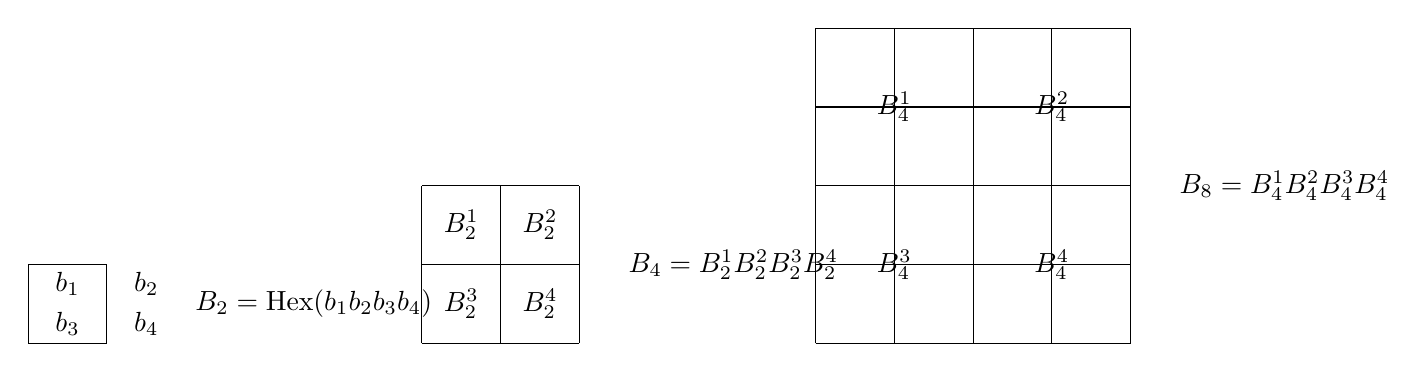
\begin{tikzpicture}
    % First block B2
    \draw (0,0) grid (1,1);
    \node at (0.5,0.75) {$b_1$};
    \node at (1.5,0.75) {$b_2$};
    \node at (0.5,0.25) {$b_3$};
    \node at (1.5,0.25) {$b_4$};
    \node[right] at (2,0.5) {$B_2 = \text{Hex}(b_1b_2b_3b_4)$};

    % Second block B4
    \begin{scope}[xshift=5cm]
        \draw (0,0) grid (2,2);
        \node at (0.5,1.5) {$B_2^1$};
        \node at (1.5,1.5) {$B_2^2$};
        \node at (0.5,0.5) {$B_2^3$};
        \node at (1.5,0.5) {$B_2^4$};
        \node[right] at (2.5,1) {$B_4 = B_2^1 B_2^2 B_2^3 B_2^4$};
    \end{scope}

    % Third block B8
    \begin{scope}[xshift=10cm]
        \draw (0,0) grid (4,4);
        \node at (1,3) {$B_4^1$};
        \node at (3,3) {$B_4^2$};
        \node at (1,1) {$B_4^3$};
        \node at (3,1) {$B_4^4$};
        \node[right] at (4.5,2) {$B_8 = B_4^1 B_4^2 B_4^3 B_4^4$};
    \end{scope}
\end{tikzpicture}

\end{document}